\chapter{論理・集合・記号}\label{chapt_logic}

{\small ここで学ぶ内容の多くは, ある意味, 直感的に「当たり前」のことである。
しかし, 当たり前のことが, 数学では, 注意深く選ばれ, 注意深く定義されていること
に注意してほしい。これらの「当たり前」のことを土台にして数学が
構築され, それを土台にして, 現代科学が構築されているのだ。\\}

\section{条件と命題}

例えば以下のようなものを, \underline{条件}\index{じょうけん@条件} (condition)と呼ぶ:
\begin{itemize}
\item 整数$n$は4の倍数である。
\item 整数$n$は偶数である。
\item ある人は筑波大生である。\footnote{ここで言う「ある人」とは, 特定の人をさしているのではない。
誰でもいいから筑波大生のひとりを想定するのだ。}
\end{itemize}
条件は, 正しいとか正しくないとかの議論, つまり真偽の議論の対象にはならない。ある人は筑波大生である, 
と言われても, 「ふーん, それで?」と思うだけだ。ところが, 条件を適当に組み合わせれば, 真偽が問われる
発言になる。それを\underline{命題}\index{めいだい@命題} (proposition)という。

「命題」は, 多くの場合, 2つの条件$p$, $q$について, 「$p$ならば$q$である」という形で表現できる。
\begin{exmpl}\label{ex:logic1}
\begin{itemize}
\item 整数$n$が4の倍数ならば$n$は偶数である。
\end{itemize}
という命題は, \\
  条件$p$: 「整数$n$は4の倍数である」\\
  条件$q$: 「整数$n$は偶数である」\\
の2つの条件について, 「$p$ならば$q$である」という形の主張になっている。ちなみに, この命題は真である。
(例おわり)\end{exmpl}
\mv

命題は, 一見すると「$p$ならば$q$である」という形にはなっていないものも多い。そのような
場合は, 適宜, 言葉を補って読み替える必要がある。\mv

\begin{exmpl}
\begin{itemize}
\item 4の倍数は偶数である。
\end{itemize}
という命題は, 一見すると「$p$ならば$q$である」という形にはなっていないが, 実は上の例\ref{ex:logic1}で考えた, 
\begin{itemize}
\item 整数$n$が4の倍数ならば$n$は偶数である。
\end{itemize}
と同じことである。
(例おわり)\end{exmpl}
\mv

\begin{exmpl}\label{ex:logic2}
\begin{itemize}
\item 筑波大の学生は優秀である。
\end{itemize}
という命題は, 
\begin{itemize}
\item ある人が筑波大の学生ならば, その人は優秀である。
\end{itemize}
と同じことである。ちなみに, この命題が真か偽かは, 判定が難しい。そもそも「優秀」とは
何かという議論や, それ以上に, 君の努力にかかっているのだろう!
(例おわり)\end{exmpl}
\mv

さて, 数学では, 命題の「ならば〜〜である」を二重線の矢印"$\Longrightarrow$"で表現することになっている。
\begin{exmpl} 上の例\ref{ex:logic1}, 例\ref{ex:logic2}の命題は, それぞれ以下のように表現される:
\begin{itemize}
\item 整数$n$が4の倍数$\Longrightarrow n$は偶数
\item ある人が筑波大の学生$\Longrightarrow$その人は優秀
\end{itemize}
(例おわり)\end{exmpl}
\vv


\section{条件の否定}

次に, 条件の「否定」というものを考える。ある条件の否定とは, 
「その条件が成り立たないこと」という条件である。例えば, 
条件「整数$n$は偶数」の\underline{否定}\index{ひてい@否定}は, 
「整数$n$は偶数でない」もしくは「整数$n$は奇数」である。
一般に, 条件$p$の否定を$\overline{p}$と書く。\mv

\begin{exmpl} 「実数$x$は正である」という条件の否定は「実数$x$は0以下である」となる。(例おわり)\end{exmpl}
\begin{exmpl} 「ある人が筑波大生である」という条件の否定は「ある人が筑波大生ではない」となる。(例おわり)\end{exmpl}
\mv

ある条件と, その否定は, その組み合わせで論理的にすべての場合を含まねばならない。
つまり, その条件とその否定のどちらにもあてはまらない, という場合があってはならない。
\begin{exmpl} 「ある人が筑波大生である」という条件について, 「ある人が高校生である」
というのは否定にならない。確かに高校生は同時に筑波大生にはなれないから, 「高校生である」
と言った時点でその人が筑波大生でないことは確定する。従って, 「ある人が高校生である」
というのは「ある人が筑波大生である」の否定に含まれる。しかし, それで全ての場合を言い
尽くしているわけではない。高校生でなくてしかも筑波大生でもないという人は世の中にたくさん
いるからだ。
(例おわり)\end{exmpl}
\mv

このことから, ある条件の否定の否定は, もとの条件に戻るということが, 
直感的にわかるだろう。\\

\section{「かつ」と「または」}

複数の条件を, 「かつ」とか「または」という語でつなぐと, 新しいひとつの条件ができる。

\begin{exmpl} つくば市が, 市の予算を使って, 市の子供たちのために
素晴らしいイベントを企画するとしよう。その参加者の条件は, 
例えば, 「つくば市民で, かつ, 13歳未満である」というような
ものになるだろう。これは「つくば市民である」と「13歳未満である」
という2つの条件を「かつ」でつないだものである。

この条件にクレームがつき, 「税金の大部分は大人が払っているんだから, 
つくば市の大人が参加してもいいじゃないか」という意見と, 「けち臭いこと
言わないで, つくば市以外の子供にも来て貰ってもいいじゃないか」
という意見が大勢を占めると, 参加者の条件は「つくば市民または, 
13歳未満である」というようなものになるかもしれない。
ここで注意。「つくば市民かつ13歳未満」である人も, この条件を
満たすのだ。そもそも「または」は, いくつかの条件のうち一部を
満たせばOKということであり, 全部を満たすのでももちろんOKなのだ。(例おわり)
\end{exmpl}

複数の条件が「かつ」でつながれたような条件の否定は, それぞれの条件の否定を
「または」でつないだものになる。すなわち, 条件$p$, 条件$q$について, 
\begin{eqnarray}
\overline{p\text{かつ}q}=\overline{p}\,\text{または}\overline{q}
\end{eqnarray}
である。

\begin{exmpl} 「つくば市民で, かつ, 13歳未満である」の否定は, 
「つくば市民でない, または13歳以上である」という条件になる。(例おわり)\end{exmpl}

複数の条件が「または」でつながれたような条件の否定は, それぞれの条件の否定を
「かつ」でつないだものになる。すなわち, 条件$p$, 条件$q$について, 
\begin{eqnarray}
\overline{p\text{または}q}=\overline{p}\,\text{かつ}\overline{q}
\end{eqnarray}
である。

\begin{exmpl} 「つくば市民または, 13歳未満である」の否定は, 
「つくば市民でない, かつ, 13歳以上である」という条件になる。(例おわり)\end{exmpl}

\begin{exmpl} 「整数$n, m$はともに偶数である」という条件は, 「整数$n$は偶数であり, かつ, 
整数$m$は偶数である」という条件と同じである。したがって, その否定は, 「整数$n$は奇数
であるか, または, 整数$m$は奇数である」, すなわち, 「整数$n, m$のうち少なくとも
どちらかは奇数である」となる。(例おわり)\end{exmpl}

\begin{q}\label{q:cond0} 以下の条件の否定を述べよ:
\begin{enumerate}
\item 実数$x$は負である。
\item 実数$x$,$y$のうち, すくなくとも一方は正である。
\item 実数$x$,$y$は, 両方とも正である。
\end{enumerate}
\end{q}
\vv


\section{逆・裏・対偶}\index{ぎゃく@逆}\index{うら@裏}\index{たいぐう@対偶}

命題$p \Longrightarrow q$について, 以下のように\underline{逆}, \underline{裏}, \underline{対偶}という
命題を考えることができる:\\
 $q \Longrightarrow p$を「逆」\\
 $\overline{p} \Longrightarrow \overline{q}$を「裏」\\
 $\overline{q} \Longrightarrow \overline{p}$を「対偶」\\
と呼ぶ。

\begin{exmpl}
\begin{itemize}
\item 整数$n$が4の倍数$\Longrightarrow n$は偶数
\end{itemize}
について, 逆, 裏, 対偶は, 以下のようになる:
\begin{itemize}
\item 逆: 整数$n$が偶数であれば, 整数$n$は4の倍数である。
\item 裏: 整数$n$が4の倍数でなければ, 整数$n$は偶数でない。
\item 対偶: 整数$n$が偶数でなければ, 整数$n$は4の倍数でない。
\end{itemize}
(例おわり)\end{exmpl}

この例では, 命題とその対偶は真だが, 逆と裏は偽である。実際, $n=2$は
偶数だが4の倍数ではない。従って「逆」は偽である(反例)。$n=2$は4の倍数では
ないが, 偶数である。従って「裏」も偽である(反例)。このように, 一般に, 
ある命題の真偽と, その逆や裏の真偽は, 必ずしも一致しない。

しかし, \textgt{命題とその対偶は必ず真偽が一致する}。従って, 「対偶」は, 
命題をそのまま言い換えたものだとも言える。\\

\begin{exmpl}
\begin{itemize}
\item 筑波大の学生は優秀である。
\end{itemize}
という命題について, 逆, 裏, 対偶は, 以下のようになる:
\begin{itemize}
\item 逆: 優秀であれば筑波大の学生である。
\item 裏: 筑波大の学生でなければ優秀でない。
\item 対偶: 優秀でなければ筑波大の学生でない。
\end{itemize}
(例おわり)\end{exmpl}
\mv


\begin{q}\label{q:logic_gyaku0} 以下の命題の逆, 裏, 対偶をそれぞれ述べよ(真偽は問わない)。
\begin{enumerate}
\item $x=0$ならば$x^2=0$である。
\item $x>0$ならば$x^2>0$である。
\item 強いものは勝つ。
\end{enumerate}
\end{q}
\mv


\begin{q}\label{q:logic_taigu0} 以下のことわざ・名言の対偶をそれぞれ述べよ(真偽は問わない。なお, 
(3)は映画監督の宮崎駿の言葉)。
\begin{enumerate}
\item 良薬は口に苦し。
\item 能ある鷹は爪を隠す。
\item 大事な事はめんどくさいものである。
\end{enumerate}
\end{q}
\vv


\section{命題の否定}\index{ひてい@否定}

ある命題が偽であることを示す, つまり命題を\underline{否定}するにはどうすればいいだろうか? 
一般に, 命題「$p$ならば$q$である」の否定は, 「$p$であるのにもかかわらず$q$でない
場合が(必ず)存在する」である。

\begin{exmpl}\label{exmpl:Utsukuba_good_nogood10}
\begin{itemize}
\item 筑波大の学生は優秀である。
\end{itemize}
という命題の否定はなんだろう?
\begin{itemize}
\item 筑波大には優秀でない学生もいる。
\item 筑波大生の少なくとも1人は優秀でない。
\item 筑波大生でありながら, 優秀でない学生もいる。
\end{itemize}
などである。(例おわり)\end{exmpl}

簡単なようだが, これを間違える人が, とても多い。誤答の例を挙げよう:
\begin{itemize}
\item (誤答A) 筑波大の学生は優秀でない。
\item (誤答B) 筑波大には優秀な学生はいない
\item (誤答C) 筑波大の学生は優秀であるとは限らない。
\end{itemize}
命題の否定の否定は, もとの命題に戻らなければならないのだ。
誤答Aと誤答B(これらはともに同じ命題)をもういちど否定すると, 
\begin{itemize}
\item 筑波大には優秀な学生がいる。
\end{itemize}
となってしまうが, これは当初の「筑波大の学生は優秀である」
よりもずいぶん弱い命題になっている。つまり, 誤答Aと誤答Bは, 
あまりに否定しすぎたのだ。優秀でない人がひとりでもいれば, 
「筑波大の学生は優秀である」という命題は否定されるので
あり, すべての筑波大生について「優秀でない」という烙印を
押す必要は無かったのだ。

誤答Cは, 実際にもし筑波大の学生全員が優秀であっても
成り立つ命題である。「筑波大の学生は優秀である」という
命題について「そうではない\textgt{かもしれない}」
と言っているだけで, 「そうではない」と言いきって(否定して)
はいない。「どっちとも言い切れないように思う」
「判断材料が足りない」「ちゃんと調べるべきだ」などの
ニュアンスを含むが, 結局は何も言っていない, 玉虫色の命題だ。
なので, 科学の世界では「〜とは限らない」は禁句!\mv

「すべての...は〜〜である」とか, 「どんな...も〜〜である」という命題の否定は, 
「〜〜でないような...も存在する」である。\\

\begin{exmpl}
「すべての鳥は飛べる」とか「どんな鳥も飛べる」の否定は, 
「飛べない鳥も存在する」である。
(例おわり)\end{exmpl}

一方, 「〜〜であるような...が存在する」の否定は, 
「どんな...も〜〜でない」となる。
\begin{exmpl}
「白雪姫」での鏡の発言:
\begin{itemize}
\item 王妃よりも美しい人が存在する。
\end{itemize}
の否定は, 以下のようになる。
\begin{itemize}
\item どんな人も, 王妃より美しくはない。
\end{itemize}
(例おわり)\end{exmpl}
\mv

結論が否定形になるような命題は, 気をつけないと曖昧になる。

\begin{exmpl}
\begin{itemize}
\item すべての関西人は納豆好きではない。
\end{itemize}
という命題は, 
\begin{itemize}
\item 『すべての関西人は納豆好き』ではない。
\item 『すべての関西人』は『納豆好きではない』。
\end{itemize}
というふうに, 2通りに解釈できる。前者は, 納豆好きの関西人がいる可能性
も残す「部分否定」だが, 後者は, 関西人に納豆好きはいないという「全否定」
である。このような, 2通りに解釈ができる表現は誤解やトラブルの元
なのでダメ!「すべての...は〜〜ではない」という表現は危険なので, 数学だけでなく, 
どんな場所でも使わないようにしよう。(例おわり)\end{exmpl}
\mv

\begin{exmpl}
\begin{itemize}
\item 偶数ならば4の倍数でない。
\end{itemize}
という命題は, 
\begin{itemize}
\item 偶数ならば『4の倍数でない』。
\item 『偶数ならば4の倍数』でない。
\end{itemize}
というふうに, 2通りに解釈できる。前者は, 偶数であるというだけで無条件に
『4の倍数でない』と言える, という意味であり, これは偽だ。例えば8は偶数
だが4の倍数でもある。後者は, 「偶数ならば4の倍数」という命題は偽である, 
すなわち, 偶数であっても4の倍数でないことがある, という意味であり, 
これは真である。(例おわり)\end{exmpl}
\mv

%グループは「ポケモンGOの健康への影響は穏やかなようだ。多くの身体活動への介入のように、歩数の増加は続かなかった」と結論づけている。


\begin{q}\label{q:logic_hitei0} 以下の「」内で示された命題の, 
否定を述べよ。真偽は問わない。
「〜〜わけではない」「〜〜とは限らない」という答えはダメ。
\begin{enumerate}
\item 春になると, 雪が融ける。
\item 筑波大に入れば, 素晴らしい将来が約束される。
\item どんな数も, 2乗したら0以上になる。
\item 2乗したら負になるような数は存在しない。
\end{enumerate}
\end{q}
\mv


\begin{q}\label{q:logic_soccer0}
命題「筑波大生は, みな, サッカーがうまい。」の否定は次のうちどれか? 正解は1つとは限らない。
\begin{enumerate}
\item 筑波大生は, みな, サッカーが下手。
\item 筑波大以外の学生は, サッカーが下手。
\item 筑波大以外の学生は, サッカーがうまい。
\item 筑波大以外にもサッカーがうまい学生はいる。
\item 筑波大生の何人かはサッカーがうまい。
\item 筑波大にはサッカーの下手な学生がいる。
\item 筑波大にはサッカーのうまい学生がいる。
\item 筑波大生のほとんどはサッカーが下手。
\item 筑波大生は, みな, サッカーがうまいとは限らない。
\end{enumerate}
\end{q}
\mv


ある命題が偽であることを証明する場合, \underline{反例}\index{はんれい@反例}を挙げれば済むことが多い。

\begin{exmpl}
「すべての鳥は飛べる」の否定は「飛べない鳥もいる」なので, 反例として, 
実際に飛べない鳥の具体例を挙げればよい。どんな鳥だって生まれた
ばかりのヒナは飛べないし, ニュージーランドのキウィは成鳥でも飛べない。
そういう例をひとつでも挙げることができれば, 「すべての鳥は飛べる」
という主張は粉砕されるのだ。
(例おわり)\end{exmpl}
\mv

しかし, 反例を挙げるという作戦が通用しない命題もある。\\
\begin{exmpl}
「宇宙人は存在する」というような命題が偽であると証明するのは難しい。これは反例で示すことは
できない。宇宙人が存在することを示すには, どこかから一人の宇宙人を連れてくればいいのだが, 存在しない
ことを示すには, 広大な宇宙のどこにも宇宙人が存在しないことを示さねばならない。
(例おわり)\end{exmpl}
\mv

反例を挙げる場合は, それが反例になっている, ということまで踏み込んで説明する必要がある。

\begin{exmpl}
「2桁の整数は必ず3で割り切れる」というような命題が偽であることを, 反例を挙げて証明しよう。
よくあるのが, 「反例として11がある。以上。」みたいな解答である。しかし, 
ちゃんとやるなら, 「$11=3\times3+2$なので, 11を3で割ると2余る。すなわち11は2桁の
整数なのに3では割り切れない」と書くべきである。(例おわり)\end{exmpl}

この例のような簡単な問題なら, ここまでくどく書かなくてもOKかもしれない。
どこまでくどく説明すべきかは, 問題や状況による。大事なのは, 「自分は
この問題をちゃんと理解し, 解きましたよ」ということを, 自分自身や他人に説得力
を持って説明する, ということである。一目で明らかであるような簡単な状況を
除いて, それが反例になっている, ということまで説明しないと, 相手は納得して
くれない。\\

\begin{q}\label{q:logic_square0}
命題「どんな実数も, 2乗すれば正(0より大)になる」が偽であることを, 反例で証明せよ。
\end{q}
\vv



\section{必要条件・十分条件}\index{ひつようじょうけん@必要条件}\index{じゅうぶんじょうけん@十分条件}

さて, いま, 命題
\begin{eqnarray}p \Longrightarrow q\end{eqnarray}
が成り立つ(真である)としよう。このとき, 条件$q$が成り立つにはとりあえず条件$p$が成り立てば十分なので, 
条件$p$は条件$q$の\underline{十分条件}と言う。

一方, 条件$p$が成り立つなら条件$q$は必ず成り立つ。この対偶は, 「$q$が成り立たなければ
$p$は成り立たない」となる(ここでは$p$が原因で$q$が結果, みたいな因果関係は忘れて考えている)。
つまり, $q$が成り立つということは, $p$が成り立つためには必ずクリアしなければならない条件
である。そこで, 条件$q$は条件$p$の\underline{必要条件}という。

簡単に言うと, 二重線矢印"$\Longrightarrow$"の根元に来るのが十分条件で, 先に来るのが必要条件である。\\

「$p$ならば$q$」と, その逆, すなわち「$q$ならば$p$」が, ともに成り立つ場合, $p$は$q$の十分条件でもあり, 
必要条件でもある。このような場合, $p$は$q$の\underline{必要十分条件}\index{ひつようじゅうぶんじょうけん@必要十分条件}
である, といい, 以下のように表現する:
\begin{eqnarray}p \Longleftrightarrow q\end{eqnarray}
$p$が$q$の必要十分条件であれば$q$は$p$の必要十分条件になるので, $p$と$q$は実質的に同じ条件である。そこで, 
$p$と$q$は\underline{同値}\index{どうち@同値}である, ともいう。\\

\begin{q}\label{q:logic_hitsuyo0}
以下の条件$p, q$について, $p$は$q$の必要条件か, 十分条件か, 必要十分条件か, そのいずれでもないか, 述べよ。\\
$p$: 実数$x$について, $x^2=1$である。\\
$q$: 実数$x$は1に等しい。
\end{q}
\mv


\begin{q}\label{q:logic_hitsuyo1} 
以下の条件$p, q$について, $p$は$q$の必要条件か, 十分条件か, 必要十分条件か, そのいずれでもないか, 述べよ。\\
$p$: 実数$x$について, $x^2=1$である。\\
$q$: 実数$x$は$-2$より大きい。
\end{q}
\mv

ところで, 日本語の表現として, 「AはBである」と言うときと, 「AとはBである」と言うときの
違いを考えよう。
\begin{exmpl}\label{ex:to_toha}
「人間は動物である」と「人間とは動物である」は意味が違う。前者は正しく, 
後者は誤り。前者は「(人間以外の動物もいるかもしれないがともかく)人間は動物の一種である」
という意味だが, 後者は「人間と動物は同じである」という意味である。
(例おわり)\end{exmpl}
\mv

このように, 「AはBである」は, 多くの場合, 「AならばBである」と同じ意味である。
すなわちBはAの必要条件である。一方, 「AとはBである」と言うときはAとBが同値
(互いに必要十分条件)である。

日常的・直感的な話ならば, これらの違いはあまり問題
にならないが, 話が込み入ってくると, この違いが曖昧になり, 論理が崩れることがある。
また, 文学的・修辞的・比喩的な強調表現として例えば「人生とは旅である」
「教育とは愛である」のようなものは, 論理操作に耐えるような命題ではないので, 
気をつける必要がある。

授業や試験でよく出てくる「〜〜とは何か?」という問は, 断片的な必要条件や, 文学的・
比喩的な表現を問うのではなく, 「〜〜」を過不足なく説明するもの, つまり「〜〜」の
必要十分条件で, なおかつ「〜〜」よりもわかりやすいものを問う。それは多くの場合, 
「〜〜」の定義である。\\

\begin{exmpl}
人生とは何か? 人が生まれてから死ぬまでの間のこと。
(例おわり)\end{exmpl}

\begin{exmpl}
ヘリウムとは何か? 「元素の一種である」というのは良い答えではない。
「元素の一種である」ような存在は, ヘリウム以外にもたくさんある。
(例おわり)\end{exmpl}
\mv

定義の中で使われる言葉や概念は, 自明なものか, もしくは既に定義されたもので
なければならない。よくある間違いは, 「〜〜」の定義に「〜〜」自体を使って
しまうことである(循環論法)。\\

\begin{exmpl}
無理数とは何か? 「有理数でない実数」というのは良い答えではない。こう言うためには, 
無理数を含めた「実数」を定義する必要があるからである。
(例おわり)\end{exmpl}

\begin{exmpl}
微分係数とは何か? 「接線の傾き」というのは良い答えではない。こう言うためには, 
「接線」を定義する必要があるが, それには(視覚的な直感に訴えない限り)微分係数
の概念が必要だからである。
(例おわり)\end{exmpl}
\mv

こういうことを言い始めたら, きりが無いように思える。そう, 学問はそのような
ものなのだ。「〜〜とは何か?」という問を, どこまでも厳しく問い詰めていく, 
きりの無い作業なのだ。\\

\begin{q}\label{q:logic_human_animal}
人間と動物はどう違うか?
\end{q}
\vv

\section{背理法}

命題の証明の仕方のひとつに\underline{背理法}\index{はいりほう@背理法}がある。これは, 命題の結論を
仮に否定してみると, どこかに矛盾が生じてしまう, という論法である。

\begin{exmpl}
命題「筑波大生は優秀である」を背理法で証明(?)してみよう: 

ある筑波大生が優秀でないと仮定しよう。筑波大の入試は優秀でなければ合格できない。ところが, 
その人が筑波大生であるということは, 優秀でない人が入試に合格したということになる。これは矛盾
である。従って, 筑波大生は優秀である。(証明?終わり)\\

むろん, この「証明?」は, 別の意味で不完全であり, ほんとうの証明にはなっていない。先に述べた
ように「優秀」とはどういうことかという定義があいまいだし(だからこそいろんな入試があるのだ), 
何よりも, 人は時間によってかわるものであり, 人生のある時期に「優秀」だからといって, その後も
そうであり続ける保証はない。
(例おわり)\end{exmpl}
\mv

もうひとつの例をやってみよう。こんどは厳密な証明である。\\

\begin{exmpl}
自然数$n$について, もし$n^2$が偶数ならば, $n$は偶数である。これを背理法で証明しよう。

$n^2$が偶数でありながら, $n$が偶数でない, つまり$n$は奇数であると仮定する。
すると, $n$は2を約数に持たないので, $n^2$も2を約数に持たない。従って, $n^2$は奇数になる。
これは矛盾である。従って, $n$は偶数である。\qed
(例おわり)\end{exmpl}
\mv

%賢明な君は, 背理法は「対偶の証明」に他ならないことに気づいただろうか? 

\begin{q}\label{q:logic_oddeven0}
自然数$n$について, もし$n^2$が奇数ならば, $n$は奇数である。これを背理法で証明せよ。
\end{q}
\mv

\begin{q}\label{q:logic_oddadd}
2つの自然数$n, m$について, もしそれらの積$nm$が奇数ならば, $n, m$はともに奇数である。
これを背理法で証明せよ。
\end{q}

\begin{freqmiss}{\small\textgt{↑この問題の解答を, "自然数$n, m$が
ともに偶数であると仮定する"というふうに始めてしまう} ... そういう人は, 
\pref{chapt_logic}から真剣に読み返すべきです。}\end{freqmiss}\mv

\begin{freqmiss}{\small\textgt{↑この問題の解答を, "もし$nm$が偶数ならば"
というふうに始めてしまう} ... 話がズレています。$nm$が偶数のときなんか話題に
なっていません。}\end{freqmiss}\mv

\begin{freqmiss}{\small\textgt{↑この問題の解答を, "自然数$n, m$に
ついて, もしそれらの積$nm$が奇数ならば, $n, m$のどちらかは偶数であると仮定する"
というふうに始めてしまう} ... これ, 多くの資源生がやらかします。丁寧に書こうとして, 
かえって間違っています。正しいのは, "自然数$n, m$について, もしそれらの
積$nm$が奇数\textgt{でありながら}, $n, m$のどちらかは偶数である
(\textgt{ような場合がある})と仮定する"です。違いはわかりますか?}\end{freqmiss}\mv

\begin{faq}{\small\textgt{↑これ, よくわかりません}... 
"もしそれらの積$nm$が奇数ならば, $n, m$のどちらかは偶数であると仮定する"
と始めて, 矛盾が導かれたとしましょう。それは, この仮定した命題が偽である, 
ということですよね。そこから言えるのは, 「$nm$が奇数でありながら$n, m$のいずれもが
奇数であるような場合が存在する」ということです。それはここで証明したかった
命題よりもずいぶん弱い命題です。}\end{faq}


背理法の論理は, いずれ統計学で「仮説検定」「帰無仮説」という考え方で使うことになる
ので, しっかり理解しよう。\\

% sqrt{2}が無理数であることの証明

% \section{証明のコツ}
% 自己完結性
% 「それぞれ」と「互いに」
% あいまいな言葉で自分をごまかしていないか? (わかった気になってないか?)



\section{集合}\index{しゅうごう@集合}

ものの集まりを, \underline{集合}(set)という(定義)。ここでいう「もの」とは, 
具体的な物体でもよいし, 抽象的な概念(頭の中でしか想像できないもの)でもよい。

\begin{exmpl}\label{ex:group12}
\begin{eqnarray}
S=\{\text{{\small 赤木剛憲, 三井寿, 宮城リョータ, 流川楓, 桜木花道}}\}\nonumber\\\label{eq:alg_ex_set}
\end{eqnarray}
で定義される集合$S$は, 漫画「スラムダンク」\footnote{作者は井上雄彦。少年ジャンプに1990年から1996年に連載。}
の湘北高校バスケットボール部のスターティングメンバーの集まり(スターティングファイブ)である。(例おわり)\end{exmpl}
\mv

集合を構成する個々の「もの」を, その集合の\underline{要素}\index{ようそ@要素}
\footnote{元\index{げん@元} (げん)ともいう。}(element)という(定義)。例えば例\ref{ex:group12}では, 
赤木剛憲\footnote{湘北高校バスケ部の主将。代表的な発言は, 
「基本がどれほど大事かわからんのか!! ダンクができようが何だろうが, 
基本を知らん奴は試合になったら, 何もできやしねーんだ!!」}は$S$の要素である。
ある集合を定義するときは, \eref{eq:alg_ex_set}のように, その要素を$\{\, \}$で囲って列挙すればよい。

要素をすべて列挙するのが面倒な場合は, 
$\{\, \}$の中を$|$で区切って, その右に条件を書いたりする。

\begin{exmpl}\label{ex:group3}
正の偶数からなる集合$B=\{2, 4, 6, 8, \cdots\}$は, 
\begin{eqnarray}
B=\{2n\,|\,n \text{は1以上の整数}\}
\end{eqnarray}
と表すことができる\footnote{ここで$n$は便宜上1以上の整数を表すものであり, それを記号$n$で表したこと
には何の必然性もない。$B=\{2m\,|\,m \text{は1以上の整数}\}$と書いても, 全く同じことである。もちろん, 
「1以上の整数」のかわりに「自然数」と書いてもOK。}。
(例おわり)\end{exmpl}
\mv

\begin{q}\label{q:alg_set_def}
集合とは何か? 要素とは何か? それらの定義を述べよ。
\end{q}\mv

あるもの$x$が, ある集合$X$の要素であるということを, 以下のように表記する:
\begin{eqnarray}x \in X\label{eq:algebra_set5}\end{eqnarray}
又は以下のように書いてもよい(\eref{eq:algebra_set5}と同じ意味):
\begin{eqnarray}X \ni x\end{eqnarray}
例えば例\ref{ex:group12}では, $\text{赤木剛憲} \in S$などとなる。\\

あるもの$x$が, ある集合$X$の要素でないときは, 以下のように書く:
\begin{eqnarray}x \notin X\end{eqnarray}
例えば例\ref{ex:group12}では, $\text{赤木晴子} \notin S$
となる\footnote{赤木剛憲の妹。主人公桜木花道をバスケ部にリクルートし, 桜木の精神的支柱となる。
代表的な発言は, 「地道な努力はいつか必ず報われるって, お兄ちゃんがいってたわ。」}。\\

\begin{freqmiss}{\small\textgt{点(.)とコンマ(,)をきちんと書き分けできない。
例えば, 1.2と2.3という2つの数からなる集合$\{1.2,\, 2.3\}$を, 
$\{1.2.\, 2.3\}$というふうに書いてしまう。}}\end{freqmiss}


注意: 「もの」と「ものの集まり」の違いをしっかり区別しよう。例えば, 
1と$\{1\}$は違う。前者は1という数のことだが, 後者は, 「1という数だけ
からなる集合」である。
\begin{eqnarray}
0\notin \{1\}
\end{eqnarray}
という式は意味があるが(あるもの(数)がある集合の要素かどうか), 
\begin{eqnarray}
0\notin 1
\end{eqnarray}
という式は意味がない(もの(数)がもの(数)の要素かどうかという概念は存在しない)。
\begin{eqnarray}
0 < 1
\end{eqnarray}
という式は意味があるが(数どうしの間には大小関係がある), 
\begin{eqnarray}
0< \{1\}
\end{eqnarray}
という式は意味がない(数と集合の間に大小関係は無い)。
\\

ある集合$X$の全ての要素が, 別の集合$Y$の要素でもあるときは, 「集合$X$は集合$Y$に
含まれる」とか, 「$X$は$Y$の\underline{部分集合}\index{ぶぶんしゅうごう@部分集合}
(subset)である」, と言い, 以下のように書く(定義):
\begin{eqnarray}X \subset Y\label{eq:subset001}\end{eqnarray}
又は以下のように書いてもよい(\eref{eq:subset001}と同じ意味):
\begin{eqnarray}Y \supset X\end{eqnarray}

\begin{exmpl} $S$を筑波大学生物資源学類生全員の集合とし, $S_1$を筑波大学生物資源学類の
1年生全員の集合とする。$S_1$の全ての要素は, $S$の要素でもある。従って$S_1\subset S$である。
(例おわり)\end{exmpl}
\mv

\begin{q}\label{q:alg_subset001}
集合$X$が集合$Y$に含まれる(集合$X$が集合$Y$の部分集合である)とはどういうことか, 定義を述べよ。
\end{q}\mv

\begin{freqmiss}{\small\textgt{$\in$と$\subset$を混同してしまう} ... 
これらは違う意味を持つ記号です。}\end{freqmiss}

部分集合の定義から明らかなように, どのような集合も, 自分自身の部分集合である。
つまり任意の集合$X$について, 
\begin{eqnarray}
X \subset X
\end{eqnarray}
である。

集合$X$と集合$Y$が, $X\subset Y$かつ$X\supset Y$であるとき, すなわち, 
$X$が$Y$に含まれ, $Y$が$X$に含まれるとき, $X$と$Y$は\underline{一致する}と言い,
以下のように書く:
\begin{eqnarray}
X = Y
\end{eqnarray}
\mv

\begin{q}\label{q:logic_subset0} 以下の式について, 間違っているものを, 理由とともに指摘せよ:
\begin{edaenumerate}
\item $1\in\{1, 2, 3\}$
\item $1\subset\{1, 2, 3\}$
\item $\{1\}\in\{1, 2, 3\}$
\item $\{1\}\subset\{1, 2, 3\}$
\item $\{1, 2\}\in\{1, 2, 3\}$
\item $\{1, 2\}\subset\{1, 2, 3\}$
\item $\{1, 2, 3\}\subset\{1, 2, 3\}$
\end{edaenumerate}
\end{q}
\mv

2つの集合$X$, $Y$に共通する要素だけを抜き出してできる集合を, \underline{積集合}とか
\index{せきしゅうごう@積集合}\underline{共通部分}\index{きょうつうぶぶん@共通部分}
とか\underline{交わり}\index{まじわり@交わり}といい, 以下のようにあらわす:
\begin{eqnarray}
X \cap Y
\end{eqnarray}

\begin{exmpl}
\begin{eqnarray}
\{1, 2, 3\} \cap \{2, 3, 4\}=\{2, 3\}
\end{eqnarray}
(例おわり)\end{exmpl}
\mv

2つの集合$X$, $Y$の少なくとも一方に属する要素でできる集合を, \underline{和集合}\index{わしゅうごう@和集合}
とか\underline{結び}\index{むすび@結び}といい, 以下のようにあらわす:
\begin{eqnarray}
X \cup Y
\end{eqnarray}

\begin{exmpl}
\begin{eqnarray}
\{1, 2, 3\} \cup \{2, 3, 4\}=\{1, 2, 3, 4\}
\end{eqnarray}
(例おわり)\end{exmpl}
\mv

要素が一つもない集合を\underline{空集合}\index{くうしゅうごう@空集合}といい, $\varnothing$であらわす。
\begin{exmpl}
\begin{eqnarray}
\{1, 2, 3\} \cap \{4, 5, 6\}=\varnothing
\end{eqnarray}
(例おわり)\end{exmpl}
\mv

数学では, 慣習的に, よく使う集合に特別な記号がつけられている。例えば, 
\begin{itemize}
\item $\mathbb{N}$ 「自然数全体の集合\footnote{自然数は, 正の整数である。0は含まない。}」
\item $\mathbb{Z}$ 「整数全体の集合」
\item $\mathbb{Q}$ 「有理数全体の集合」
\item $\mathbb{R}$ 「実数全体の集合」
\item $\mathbb{C}$ 「複素数全体の集合」
\end{itemize}
である。当然, 
\begin{eqnarray}
\mathbb{N} \subset \mathbb{Z} \subset \mathbb{Q} \subset \mathbb{R} \subset \mathbb{C}
\end{eqnarray}
である\footnote{複素数は, 2つの実数$x, y$によって$x+iy$と書ける数である。従って, 
$y=0$のとき, すなわち, 任意の実数$x$も, 複素数である。むろん, $x=y=0$のとき, 
つまり$0$も, 複素数である}。

%\begin{faq}{\small\textgt{無理数全体の集合の記号は無いのですか?}
%... 私は見たことありません。}\end{faq}

これらを使うと, 数学の記述が簡潔になって, 楽である。例えば, 
\begin{eqnarray*}x\in\mathbb{R}\end{eqnarray*}
は「$x$は実数全体の集合の要素である」ということなのだが, それは要するに「$x$は実数である」
ということだ。従って, 「$x$は実数である」という記述を$x\in\mathbb{R}$と記述してしまっても
かまわない。\\

\begin{q}\label{q:logic_group_elem0}
以下の集合を, 要素を列挙する形で表せ。
\begin{enumerate}
\item $\{2n\,|\,n \in \mathbb{N}\}$
\mv
\item $\{2n-1\,|\,n \in \mathbb{N}\}$
\mv
\item $\{-1, 0, 1, 2, 3\} \cap \mathbb{N}$
\mv
\item $\{n^2\,|\,n\in\mathbb{Z}\} \cap \{x\,|\,-5<x<5, x\in\mathbb{R}\}$
\end{enumerate}
\end{q}
\mv

さて, ある大きな集合を前提として, その中に含まれる部分集合についていろいろ考えることがある。
\begin{exmpl}
あるサッカークラブが試合に臨むときは, そのクラブに属する選手の中の11人がスターティングメンバー
(スタメン)としてピッチに立ち, さらに7人ほどが交代要員としてベンチ入りする
(それ以外の選手はスタンドで観戦する)。スタメン決定は, そのクラブの選手全員からなる
集合(上述した「大きな集合」)の中でどのように「スタメン」と「交代要員」
という2つの部分集合を作るかという話に他ならない
\footnote{ただし, 誰をどのポジションに配置するかは考えない。}。
(例おわり)\end{exmpl}
\mv

そのような「大きな集合」を\underline{全体集合}\index{ぜんたいしゅうごう@全体集合}とか
\underline{普遍集合}\index{ふへんしゅうごう@普遍集合}
と呼び, 慣習的に$U$という記号\footnote{universeの頭文字。}で表すことが多い。

全体集合$U$の部分集合$A$について, $A$には含まれないような$U$の要素の
集合を$A$の\underline{補集合}\index{ほしゅうごう@補集合}と呼び, 
$\overline{A}$と表す\footnote{$^cA$と表すこともある。cはcomplementaryの頭文字。}。つまり, 
\begin{equation}\overline{A}:=\{x\,|\, x\in U\text{かつ}\,x \notin A\}\end{equation}
である(定義)。\\

\begin{exmpl} $U$を筑波大学生物資源学類生全員の集合とする。$A$を, 筑波大学生物資源学類の女子学生全員の集合
とすると, $A\subset U$であるのは当然である。また, $\overline{A}$は, 同学類の男子学生全員の集合である。
(例おわり)\end{exmpl}
\mv

\begin{exmpl} $U=\{1, 2, 3, 4, 5, 6\}$とする。ここで, $A=\{2, 3, 4\}$とする。$A$の要素は全て$U$の
要素なので, $A\subset U$である。また, $\overline{A}=\{1, 5, 6\}$である。
(例おわり)\end{exmpl}
\mv

\begin{exmpl} $U=\mathbb{N}$とする。ここで, $A$を2以上の偶数の集合とすると, $A$の要素は全て$U$の
要素なので, $A\subset U$である。また, $\overline{A}$は1以上の奇数の集合である。
(例おわり)\end{exmpl}
\mv

このような集合の包含関係は, 図\ref{fig:ven1}のような\underline{ベン図}と呼ばれる図で概念的に表すことが多い。

\begin{figure}[ht]
    \centering
    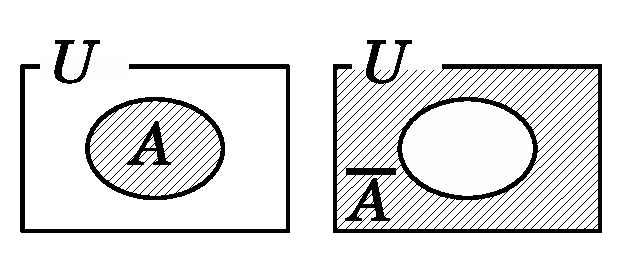
\includegraphics[width=7cm]{ven1.eps}
    \caption{ベン図。左は$A\subset U$, 右(の斜線部)は$A$の補集合(つまり$\overline{A}$)をあらわす。\label{fig:ven1}}
\end{figure}


全体集合$U$と, その部分集合$A$, $B$について, \textgt{ド・モルガンの法則}\index{どもるがんのほうそく@ド・モルガンの法則}
と呼ばれる以下の定理が成り立つ:
\begin{equation}\overline{A\cap B}=\overline{A}\cup\overline{B}\label{eq:deMorgan1}\end{equation}
\begin{equation}\overline{A\cup B}=\overline{A}\cap\overline{B}\label{eq:deMorgan2}\end{equation}
\eref{eq:deMorgan1}は, 図\ref{fig:ven2}のようなベン図を使えば, 直感的にわかるだろう。

\begin{figure}[ht]
    \centering
    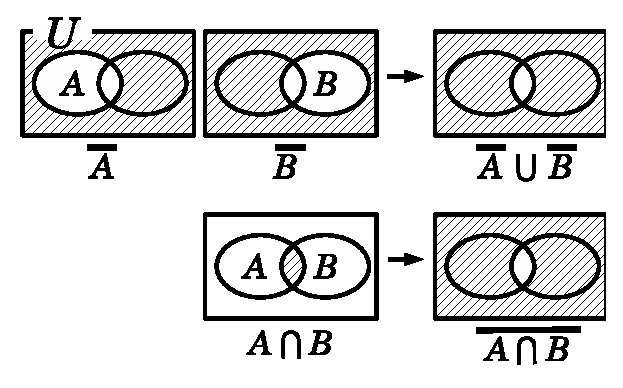
\includegraphics[width=7cm]{ven2.eps}
    \caption{\eref{eq:deMorgan1}を説明するベン図。\label{fig:ven2}}
\end{figure}
\mv

\begin{q}\label{q:logic_ben0}
ベン図を描いて, \eref{eq:deMorgan2}を説明せよ。
\end{q}
\vv


\section{集合の直積}

%\begin{itembox}{直積の定義}
2つの集合$X$, $Y$について, それぞれからひとつずつ要素をとりだしてペアを
作ることを考える。このペア全体の集合を, 
$X$と$Y$の\underline{直積}\index{ちょくせき@直積}と言って, $X \times Y$
と書く。すなわち, 
\begin{eqnarray}
X \times Y:=\{(x, y)\,|\, x\in X, y \in Y\}
\end{eqnarray}
である。
%\end{itembox}
\mv

\begin{exmpl}\label{ex:gprod1}
$A=\{1, 2\}$, $B=\{5, 6, 7\}$なら, 
\begin{eqnarray}
A \times B&=&\{1, 2\}\times\{5, 6, 7\}\nonumber\\
&=&\{(1, 5), (1, 6), (1, 7), (2, 5), (2, 6), (2, 7)\}\nonumber\\
\end{eqnarray}
である。(例おわり)\end{exmpl}
\mv

\begin{q}\label{q:logic_direct_product}
直積の定義を述べよ。
\end{q}
\mv

\begin{itembox}{注意}
直積は, 要素どうしの掛け算ではない。
\end{itembox}
初学者は, 「積」という言葉の語感から, 「直積」といえば何か「掛け算」をするものだと
感じるかもしれないが, そんなことはない。直積の式に$\times$という記号があるが, 
これは数の掛け算の記号と同じ形をしていても意味は全く別物である。単に, 可能な
\textgt{ペア}を全て集めてできる集合が直積である。なぜそうなのか? 理由は無い。
直積とはそういうものだと約束(定義)するのだ。\\

なので, 次の例のように, 別に数の集合でなくても, 直積を考えることができる:

\begin{exmpl}
\begin{eqnarray}
&&M=\{\text{ピザ, スパゲティ}\}\\
&&D=\{\text{コーヒー, 紅茶}\}
\end{eqnarray}
であれば,
\begin{eqnarray}
M \times D=&&\{(\text{ピザ, コーヒー}), (\text{ピザ, 紅茶}), \nonumber\\
&&(\text{スパゲティ, コーヒー}), (\text{スパゲティ, 紅茶})\}\nonumber\\
\end{eqnarray}
となる。これは, どこかの喫茶店の「ドリンクつきランチセット」の選択肢だろう。
(例おわり)\end{exmpl}
\mv

\begin{freqmiss}{\small\textgt{直積を「要素どうしを掛け算すること」だと誤解する。例\ref{ex:gprod1}を, 
\begin{eqnarray*}A\times B=\{5, 6, 7, 10, 12, 14\}\end{eqnarray*}
としてしまう。} ... ↑これは間違い!

直積の概念は単純明快なのに, そのような誤り(というか勝手な解釈)
をしてしまう人は, ものごとの「定義」の重要性と, そこから
始まる学問の論理性を軽視していませんか? 人間の言葉には限りが
あるので, 明解な概念であっても, それにぴったりくる言葉が無い
ことはよくあります。
そういう場合は, その概念になんとなく近い言葉を借りて代用したり
合成するしかないのです。従って, 言葉のイメージを早合点して勝手に
解釈するのは, 極めて危険です。

例えば「花吹雪」という言葉がありますが, 「吹雪」という言葉の
イメージに引きずられて, 「花の形をした雪が吹きつけること」だ, 
と勝手に解釈すると, 「花吹雪」の本当の意味(たくさんの花びらが
風でいっせいに落ち, 吹き流されて, まるで吹雪のように
見えること)とは違ってしまいます。「直積」を「要素どうしの掛け算」
と解釈する人は, そのような間違いを犯しています。}\end{freqmiss}

繰り返すが, 直積は要素どうしの積 (掛け算)ではない。
ではなぜ直「積」と呼ぶかというと, もとの集合の
\textgt{要素数(要素が何個あるか)}どうしの積(掛け算)
が, 直積の要素数になるからである。実際, 
例\ref{ex:gprod1}では, $A$の要素数は2, $B$の要素数は3で, 
$A\times B$の要素数は6になっている。\\

さて, 直積は「2つの集合」が同じ集合であってもかまわない。

\begin{exmpl}$A=\{1, 2\}$なら, 
\begin{eqnarray}
A \times A=\{(1, 1), (1, 2), (2, 1), (2, 2)\}
\end{eqnarray}
である。$(1, 2)$と$(2, 1)$を区別することに注意しよう。また, $(1, 2)$を$\{1, 2\}$
と書くのも誤りである。$(1, 2)$と$\{1, 2\}$は意味が違うことに注意しよう。すなわち, 
$(1, 2)$は1と2という数をこの順序で組み合わせたペアである(集合ではない)が, 
$\{1, 2\}$は1と2という2つの数からなる集合である\footnote{なので, 
$\{1, 2\}=\{2, 1\}$だが, $(1, 2)\neq(2, 1)$である。}。
(例おわり)\end{exmpl}
\mv

直積は, 3つ以上の集合に関しても定義される。

\begin{exmpl}3つの集合$X$, $Y$, $Z$について, 
\begin{eqnarray*}
X\times Y\times Z:=\{(x, y, z)\,|\,x\in X, y\in Y, z\in Z\}
\end{eqnarray*}
である。
(例おわり)\end{exmpl}
\mv

直積に関して, 数学や物理学で特によく使うのは, $\mathbb{R} \times \mathbb{R}$や, 
$\mathbb{R} \times \mathbb{R} \times \mathbb{R}$などである。前者は, 実数を
2つ組み合わせたものの集合, つまり, 
\begin{eqnarray}
\mathbb{R} \times \mathbb{R}=\{(x, y)\,|\,x, y \in \mathbb{R}\}
\end{eqnarray}
である。これは何か? 言うまでもなく, 2次元の数ベクトルの集合である(これは2次元の
幾何ベクトルをあらわす座標の集合でもある)。同様に, 
\begin{eqnarray}
\mathbb{R} \times \mathbb{R}\times \mathbb{R}=\{(x, y, z)\,|\,x, y, z \in \mathbb{R}\}
\end{eqnarray}
は, 3次元の数ベクトルの集合である。$\mathbb{R} \times \mathbb{R}$や, 
$\mathbb{R} \times \mathbb{R} \times \mathbb{R}$と書くのはめんどくさいので, 
かわりに$\mathbb{R}^2$や$\mathbb{R}^3$などと書く。この2とか3といった指数は, 
$2^3=8$などというときの掛け算の回数ではなくて, 直積される集合の数である。\\

\begin{q}\label{q:logic_group_elem1}
次の集合の要素を書き出せ
\begin{eqnarray}\{1, 2, 3\}\times\{2, 3, 4\}\label{eq_prob_group_product}\end{eqnarray}
\end{q}
\mv

\begin{freqmiss}{\small\textgt{直積と積集合を混同する} ... 
語感は似ているけど, これらは全く別物です。}\end{freqmiss}
\mv

\begin{q}\label{q:univ_vectprod_chokuseki} 次の\eref{eq:univ_vectprod_chokuseki1}と
\eref{eq:univ_vectprod_chokuseki2}は互いにどう違うか, 説明せよ。
\begin{eqnarray}
&&(1, 2, 3)\times(4, 5, 6)\label{eq:univ_vectprod_chokuseki1}\\
&&\{1, 2, 3\}\times\{4, 5, 6\}\label{eq:univ_vectprod_chokuseki2}
\end{eqnarray}\end{q}
\vspace{0.3cm}



\section{数学記号}\label{sect:mathsymbols}
数学やその応用分野(物理学・化学・生物学・経済学など)ではいろんな記号を使う。
さしあたって, 以下の記号を覚えておこう。この中には, 高校数学では
学ばないものも含まれるが, 「基礎数学」などの授業で
すぐに必要になるだろう。\\

\subsection*{論理と二項関係}
\begin{itemize}
\item $\forall$ 「すべての」「任意の」 ... for Allの 'A'を逆転。
\item $\exists$ 「ある」「存在する」 ... exist の 'E'を逆転。
\item $\exists!$ 「ただひとつ存在する」
\item $\Longrightarrow$ 「ならば」
\item $\Longleftrightarrow$ 「必要十分条件」「同値」
\item $\geq$ 「以上」($\geqq$は, 大学ではあまり使われない)
\item $\leq$ 「以下」($\leqq$は, 大学ではあまり使われない)
\item $=$ 「等しい」
\item $\neq$ 「等しくない」
\item $\approx$, $\fallingdotseq$ 「ほぼ等しい」
\item $\sim$ 「だいたい等しい (桁が合う程度)」「比例する」
\item $\gg$ 「はるかに大きい」
\item $\ll$ 「はるかに小さい」
\item $\propto$ 「比例する」
\item $\equiv$ 「定義する」又は「恒等的に等しい」
\item $:=$ 「定義する」
\end{itemize}

\subsection*{集合}\label{symbol_set}
\begin{itemize}
\item $\in$ (左は右の)「要素」
\item $\ni$ (右は左の)「要素」
\item $\notin$ 「要素ではない」
\item $\subset$ (左は右の)「部分集合」
\item $\supset$ (右は左の)「部分集合」
\item $\varnothing$ 「空集合」
\item $\cap$ 「共通部分」
\item $\cup$ 「和集合」
\item $\mathbb{N}$ 「自然数全体の集合」
\item $\mathbb{Z}$ 「整数全体の集合」
\item $\mathbb{Q}$ 「有理数全体の集合」
\item $\mathbb{R}$ 「実数全体の集合」
\item $\mathbb{C}$ 「複素数全体の集合」
\item $(a, b)$  $\{x|a<x<b\}$のこと。つまり, 2つの実数$a, b$で挟まれる区間\index{くかん@区間}。ただし, $a, b$は含まない。
\item $[a, b]$  $\{x|a\leq x\leq b\}$のこと。
\item $[a, b)$  $\{x|a\leq x < b\}$のこと。
\item $(a, b]$  $\{x|a< x\leq b\}$のこと。
\end{itemize}

\subsection*{演算}
\begin{itemize}
\item $\cdot$ 「掛け算」「ベクトルの内積」
\item $\bullet$ 「掛け算」「ベクトルの内積」
\item $\times$ 「掛け算」「ベクトルの外積」
\item $|\,\,|\,$ 「長さ」「絶対値」「行列式」
\item $\dot{x}\,$ 「$x(t)$を$t$で微分したもの」
\item $\bar{z}$ 「$z$の複素共役」または, 「$z$の標本平均」
\item $z^{*}$ 「$z$の複素共役」
\item $\nabla$ 「ナブラ演算子\footnote{定義は, $\nabla=(\partial/\partial x, \partial/\partial y, \partial/\partial z)$。
その意味は, 大学の数学や物理学で習う。}」
\end{itemize}

\subsection*{写像}
\begin{itemize}
\item $f: A \rightarrow B$\\「写像$f$は, 集合Aの要素を集合Bの要素に移す」(集合どうしの関係)
\item $f: a \mapsto b$\\「写像$f$は, 要素$a$を要素$b$に移す」(要素どうしの具体的な対応)
\item $g \circ f$\\「$g$と$f$の合成写像」つまり, $g\circ f: x \mapsto g(f(x))$
\end{itemize}

\subsection*{言葉の省略}
\begin{itemize}
\item i.e. 「すなわち」\index{i.e.}
\item e.g. 「例えば」\index{e.g.}
\item s.t. "such that" 「〜〜であるような」\index{s.t.}
\item cf. "compare" 「〜〜と比較せよ」\index{cf.}
\end{itemize}

\begin{faq}{\small\textgt{ファイ$\phi$って空集合の記号$\varnothing$に似ていますね。}
... 手書きのときは同じになります。}\end{faq}
\mv

\begin{faq}{\small$(a, b)$\textgt{って, ベクトルじゃないんですか?}
... おっしゃるように, ベクトルを意味することもあります。}\end{faq}
\mv

\begin{faq}{\small$(a, b)$\textgt{が集合なのかベクトルなのか, どう区別するのですか?}
... 残念ながら記号の見た目では区別できません。前後の文脈で区別します。}\end{faq}
\mv

以上の記号を使うと, 数学の論理を簡潔に表すことができる。

\begin{exmpl} 
\begin{itemize}
\item 「全ての実数$x$について, $x^2$は0以上である」
\begin{eqnarray}\forall x \in \mathbb{R}, x^2 \geq 0\end{eqnarray}
\item 「集合$A$は, 0以上の全ての整数からなる」
\begin{eqnarray}A=\{x \in \mathbb{Z}\,|\,0 \leq x\}\end{eqnarray}
\item 「自然数の集合は整数の集合に含まれる」
\begin{eqnarray}\mathbb{N} \subset \mathbb{Z}\end{eqnarray}
\item 「$x$は2以上3以下である」
\begin{eqnarray}x \in [2, 3]\end{eqnarray}
\end{itemize}
(例おわり)\end{exmpl}
\mv

\begin{q}\label{q:logic_kigou} 以下の3つの集合の違いを述べよ: 
$\{1, 2\}$と$(1, 2)$と$[1, 2]$
\end{q}
\mv


\begin{q}\label{q:logic_meidai5}
以下の命題を, 上の記号を使わないで(ただし, =と<は使ってOK)書き表せ\footnote{(2)と(3)は似ているが, 
実は全く異なる命題である。(2)は正しいが, (3)は正しくない。}。 
\begin{enumerate}
\item $x, y \in \mathbb{R}, x \propto y \Longrightarrow \exists a \in \mathbb{R}, y=ax$
\item $\forall x \in \mathbb{R}, \exists n \in \mathbb{Z}\,\,\, \text{s.t.}\,\,\, x<n$
\item $\exists n \in \mathbb{Z}\,\,\, \text{s.t.}\,\,\, \forall x \in \mathbb{R}, x<n$
\end{enumerate}
\end{q}
\mv

\begin{q}\label{q:logic_meidai6} 
以下の命題を, 上の記号を使って書き表せ:
\begin{enumerate}
\item 複素数$z$について, $z$と$z$の複素共役との和は, 実数である。
\item 実数$x$について, もし$x^2=1$ならば, $x$は$1$または$-1$である。
\end{enumerate}
\end{q}

以下は数学記号ではなく, 英語の記号だが, 呼び方を知らない人が多いので述べておく:
\begin{itemize}
\item . ドット
\item , コンマ
\item ' シングルクォート, またはアポストロフィー
\item " ダブルクォート
\item : コロン
\item ; セミコロン
\end{itemize}
特に, コロンとセミコロンを混同する人が多い。


%\begin{q}\label{q:logic_English} 以下の言葉を英訳せよ:
%\begin{edaenumerate}<3>
%\item 条件
%\item 命題
%\item 集合
%\item 要素
%\item 写像
%\end{edaenumerate}
%\end{q}\mv
\hv

\section*{演習問題}
\begin{exq}\label{q:2leq3} $2<3$という式は正しいが, $2=3$という式は正しくない。
では, $2\leq3$という式は正しいか? 正しくないか? 理由をつけて答えよ。\end{exq}

\begin{exq}\label{q:iirational_rational} 無理数と, 0でない有理数の積は, 無理数である。それを証明せよ。\end{exq}
\hv




\section*{問題の解答}

\noindent{\textbf{答}}\ref{q:cond0}
\begin{enumerate}
\item 実数$x$は0以上である。
\item 実数$x,\,y$は, どちらも0以下である。
\item 実数$x,\,y$の少なくともひとつは0以下である。
\end{enumerate}
\hv

\noindent{\textbf{答}}\ref{q:logic_gyaku0}
\begin{enumerate}
\item  逆: $x^2 = 0$ ならば, $ x = 0$である。\\
        裏: $x \neq 0$ ならば, $x^2 \neq 0$である。\\
        対偶: $x^2 \neq 0$ ならば, $x \neq 0$ である。
\mv
\item  逆: $x^2 >0$ ならば, $x>0$ である。\\
        裏: $x \leq 0$ ならば, $x^2 \leq 0$ である。\\
        対偶: $x^2 \leq 0$ ならば, $x \leq 0$ である。
\mv
\item  逆: 勝つものは, 強い。\\
        裏: 弱いものは, 負ける。\footnote{この解答では, 「勝つ」の否定は「負ける」, 「強い」の否定は「弱い」とする。現実には「引き分け」などもありうるが, 便宜上, 考えない。}\\
        対偶: 負けるものは, 弱い。
\end{enumerate}
\hv

\noindent{\textbf{答}}\ref{q:logic_taigu0} 
\begin{enumerate}
\item 苦くない薬は良薬でない(甘い薬は効かぬ)。
\item 爪を隠さないのは能ある鷹ではない(爪を見せる鷹は能無し)。
\item めんどくさくないものは大事ではない。
\end{enumerate}
\hv

\noindent{\textbf{答}}\ref{q:logic_hitei0} 
\begin{enumerate}
\item 春になっても雪が溶けないこともある(高山の万年雪など)。
\item 筑波大に入っても, 素晴らしくない将来になることもある。
\item 2乗したら負になる数が存在する。
\item 2乗したら負になる数が存在する。
\end{enumerate}
\hv

\noindent{\textbf{答}}\ref{q:logic_soccer0} 
正解は6だけ。「筑波大の学生はみなサッカーがうまい」の否定は, 筑波大生に1人でも
サッカーがうまくない人がいれば良い。1, 8は言い過ぎ。2, 3, 4は他の大学の学生のこと, つまり
関係のない話をしている。5, 7, 9は, 筑波大生全員がサッカー上手でも成り立つ。
{\small 注: 問題文で「正解は1つとは限らない」と書いてあったのに, 正解は
1つだった。君は「だまされた」と言って怒るだろうか?}
\hv

\noindent{\textbf{答}}\ref{q:logic_square0} 
 0は実数だが, 2乗したら0になる。0は正ではない。
\hv

\noindent{\textbf{答}}\ref{q:logic_hitsuyo0}
必要条件。($x=-1$という反例があるから, $p\Longrightarrow q$は成り立たない。
しかし, $q\Longrightarrow p$は成り立つ。)
\hv

\noindent{\textbf{答}}\ref{q:logic_hitsuyo1}
十分条件。($p$ならば$x=1$または$x=-1$なので$q$が成り立つ。
しかし$x=3$という反例があるから, $q\Longrightarrow p$は成り立たない。)
\hv


\noindent{\textbf{答}}\ref{q:logic_human_animal}
人間は動物の一種だが, 人間ではない動物もいる。{\small 注: 
日常の議論では「人間以外の動物」を単に「動物」と呼ぶこともある。
その場合, この設問への解答は「人間は火や道具や言葉を使うが, 
動物はそれらを使わない」等のように, 人間と, 
人間以外の動物との差異を述べることになる。このように, 
問題に現れる言葉の定義を正しく共有しないと話がかみあわない。 
真剣な議論では, くどいな, と思うくらい, 言葉の定義に
こだわらねばならないのだ。}
\hv


\noindent{\textbf{答}}\ref{q:logic_oddeven0}
$n$が奇数でない, つまり$n$は偶数であると仮定する。すると, $n$は2を約数に持つので, 
$n^2$も2を約数に持つ。従って, $n^2$は偶数になる。これは矛盾である。従って, $n$は
奇数である。\qed
\hv

\noindent{\textbf{答}}\ref{q:logic_oddadd}
自然数$n, m$のうち\textgt{少なくとも片方が}偶数であることがある
と仮定する。今, $n$が偶数なら, $n=2k$と書ける($k$は適当な自然数)。
すると$nm=2km$となる。$km$は自然数だから, $2km$すなわち
$nm$は偶数である。同様にして, $m$が偶数のときも$nm$は偶数である。
いずれにしても, $nm$は偶数になり, 矛盾する。従って, 
$n, m$はともに奇数。\qed
\hv

\noindent{\textbf{答}}\ref{q:alg_set_def} 略 (本文に書いてある)。
\mv

\noindent{\textbf{答}}\ref{q:alg_subset001} 略 (本文に書いてある)。
\mv

\noindent{\textbf{答}}\ref{q:logic_subset0} 間違っているのは, 以下の通り:\\
(2): 1は集合ではないので集合の包含関係($\subset$)は成り立たない。\\
(3): $\{1\}$は$\{1, 2, 3\}$の部分集合であり, 要素ではない。\\
(5): $\{1, 2\}$は$\{1, 2, 3\}$の部分集合であり, 要素ではない。\\
\hv

\noindent{\textbf{答}}\ref{q:logic_group_elem0}
\begin{edaenumerate}
\item $\{2, 4, 6, 8, \cdots \}$
\item $\{1, 3, 5, 7, \cdots \}$
\item $\{1, 2, 3\}$
\item $\{0, 1, 4\}$
\end{edaenumerate}
\hv

\noindent{\textbf{答}}\ref{q:logic_ben0} 図\ref{fig:ven3}参照。
\begin{figure}[ht]
    \centering
    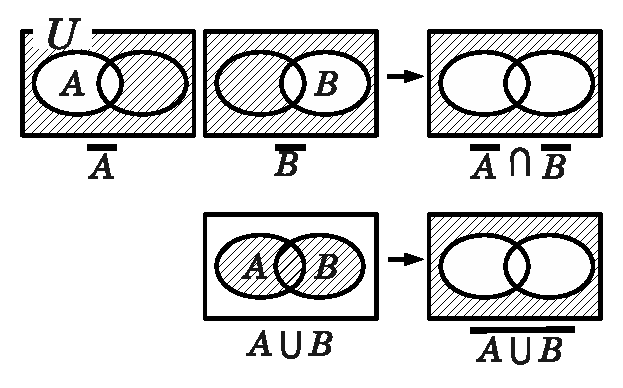
\includegraphics[width=8cm]{ven3.eps}
    \caption{\eref{eq:deMorgan2}を説明するベン図。\label{fig:ven3}}
\end{figure}

\noindent{\textbf{答}}\ref{q:logic_direct_product} 
2つの集合$X, Y$のそれぞれからひとつずつ要素を取り出してできるペアの全て
からなる集合を, $X$と$Y$の直積と言って, $X\times Y$と表す。
\hv

\noindent{\textbf{答}}\ref{q:logic_group_elem1}
 $\{(1, 2), (1, 3), (1, 4), (2, 2), (2, 3), \\(2, 4), (3, 2), (3, 3), (3, 4)\}$
\hv

\noindent{\textbf{答}}\ref{q:univ_vectprod_chokuseki}
\eref{eq:univ_vectprod_chokuseki1}はベクトルどうしの外積であり, その
結果はベクトルである。\eref{eq:univ_vectprod_chokuseki2}は集合どうし
の直積であり, その結果は集合である。すなわち, 
\begin{eqnarray*}
(1, 2, 3)\times(4, 5, 6)&=&(-3, 6, -3)\\
\{1, 2, 3\}\times\{4, 5, 6\}&=&\{(1, 4), (1, 5), (1, 6), (2, 4),\\
&& (2, 5), (2, 6), (3, 4), (3, 5), (3, 6)\}
\end{eqnarray*}
\hv

\noindent{\textbf{答}}\ref{q:logic_kigou} 略。\\

\noindent{\textbf{答}}\ref{q:logic_meidai5}
\begin{enumerate}
\item 実数$x$と実数$y$が比例するならば, ある実数$a$によって, $y=ax$と書ける。
\item どんな実数$x$にも, ある整数$n$が存在して, $x<n$とできる。(どんな実数にも, それぞれ, その実数より大きな整数がある。これは真である。)
\item ある整数$n$が存在して, どんな実数$x$にも, $x<n$とできる。(ある整数は, 全ての実数よりも大きい。これは偽である。)
\end{enumerate}
\hv

\noindent{\textbf{答}}\ref{q:logic_meidai6}
\begin{enumerate}
\item $z \in \mathbb{C}, z+\overline{z}\in\mathbb{R}$
\item $x \in \mathbb{R}, x^2=1 \Longrightarrow x = \pm 1$
\end{enumerate}

